%%%% main.tex - ACM Multimedia 2026 Dataset Track
%%%% ADS-MM: A Multimodal Cross-National Educational Resource Dataset
%%%% Uses official ACM sigconf template (single-blind)

\documentclass[sigconf,review]{acmart}

\AtBeginDocument{%
  \providecommand\BibTeX{{%
    Bib\TeX}}}

%% Rights management
\setcopyright{acmlicensed}
\copyrightyear{2026}
\acmYear{2026}
\acmDOI{XXXXXXX.XXXXXXX}

%% Conference information - ACM MM 2026 Dataset Track
\acmConference[MM '26]{Proceedings of the 34th ACM International Conference on Multimedia}{November 10--14, 2026}{Rio de Janeiro, Brazil}
\acmISBN{978-1-4503-XXXX-X/26/11}
%%\acmPrice{15.00}  % deprecated in acmart 2025+

%%
%% Additional packages
\usepackage{amsmath}
\usepackage{booktabs}
\usepackage{xspace}
\usepackage{multirow}
\usepackage{adjustbox}
\usepackage{xcolor}
\usepackage{graphicx}

%% =============================================================================
%% DATASET CONSTANTS
%% =============================================================================

% Headline
\newcommand{\HeadlineRecords}{169,000}
\newcommand{\HeadlineCourses}{27,500}

% Universities
\newcommand{\NumUniversities}{7}
\newcommand{\NumCountries}{3}
\newcommand{\NumCourses}{27,555}
\newcommand{\NumOccupations}{1,016}
\newcommand{\NumMissions}{62}
\newcommand{\NumArtifacts}{28,633}
\newcommand{\NumAttributeRecords}{140,449}
\newcommand{\NumProcessedRows}{169,082}

% Per-university
\newcommand{\NumMIT}{6,941}
\newcommand{\NumUCB}{11,076}
\newcommand{\NumStanford}{2,663}
\newcommand{\NumUIUC}{860}
\newcommand{\NumCornell}{842}
\newcommand{\NumKTH}{4,728}
\newcommand{\NumEdinburgh}{445}

% Multimodal augmentation (from collection 2026-03-31)
\newcommand{\NumOCWTotal}{2,569}          % Total OCW courses in sitemap
\newcommand{\NumOCWFetched}{1,689}        % Successfully fetched
\newcommand{\NumOCWMatched}{989}          % Matched to ADS dataset
\newcommand{\NumOCWVideo}{260}            % With video lectures (any type)
\newcommand{\NumOCWAudio}{34}             % With audio (podcasts, lecture audio)
\newcommand{\NumOCWVisual}{196}           % With visual content (image gallery, insights)
\newcommand{\NumOCWNotes}{1,100}          % With lecture notes/readings
\newcommand{\NumOCWAssessment}{843}       % With assessments
\newcommand{\NumOCWMultimedia}{396}       % With ANY multimedia (video/audio/visual)
\newcommand{\NumOCWImage}{1,689}          % With course images (cover)
\newcommand{\OCWVideoPercent}{15.4\%}     % Video percentage
\newcommand{\OCWMultimediaPercent}{23.4\%} % Any multimedia percentage
\newcommand{\OCWMatchRate}{58.6\%}        % ADS match rate
\newcommand{\MeanRichness}{1.45}          % Mean resource richness (0-6)
\newcommand{\StdRichness}{0.98}           % Std resource richness
\newcommand{\NumResourceTypes}{41}        % Distinct resource type values
% Baseline results
\newcommand{\RichnessMAE}{0.501}
\newcommand{\RichnessRho}{0.612}
\newcommand{\DeptMAE}{0.590}
\newcommand{\DeptRho}{0.430}
\newcommand{\JoinedCourses}{1,218}        % Total joined for experiments

%% Paper macros
\newcommand{\ADS}{\textsc{ADS}\xspace}
\newcommand{\ADSMM}{\textsc{ADS-MM}\xspace}
\newcommand{\todo}[1]{\textcolor{red}{\textbf{[TODO: #1]}}}

%%
%% Title
\title{ADS-MM: A Multimodal Cross-National Educational Resource Dataset for Curriculum Analysis}

%% Authors (single-blind - visible to reviewers)
\author{Author 1}
\email{author1@university.edu}
\affiliation{%
  \institution{University}
  \city{City}
  \country{Country}
}

%% CCS Concepts
\begin{CCSXML}
<ccs2012>
   <concept>
       <concept_id>10002951.10003317.10003347.10003356</concept_id>
       <concept_desc>Information systems~Multimedia information systems</concept_desc>
       <concept_significance>500</concept_significance>
   </concept>
   <concept>
       <concept_id>10002951.10003260.10003309</concept_id>
       <concept_desc>Information systems~Recommender systems</concept_desc>
       <concept_significance>300</concept_significance>
   </concept>
   <concept>
       <concept_id>10003120.10003121.10003129</concept_id>
       <concept_desc>Human-centered computing~Collaborative and social computing systems and tools</concept_desc>
       <concept_significance>300</concept_significance>
   </concept>
</ccs2012>
\end{CCSXML}

\ccsdesc[500]{Information systems~Multimedia information systems}
\ccsdesc[300]{Information systems~Recommender systems}
\ccsdesc[300]{Human-centered computing~Collaborative and social computing systems and tools}

%% Keywords
\keywords{multimodal dataset, educational resources, cross-modal analysis, curriculum benchmark, multimedia learning}

%%
%% Document
\begin{document}

%%
%% Abstract
\begin{abstract}
We present \ADSMM, a multimodal cross-national educational resource dataset spanning {\NumCourses} courses from {\NumUniversities} universities across {\NumCountries} countries (USA, Sweden, UK), augmented with structured multimedia resource annotations from MIT OpenCourseWare.
Unlike existing educational datasets that treat courses as text-only artifacts, \ADSMM captures the \emph{multimodal structure} of educational resources: which courses include video lectures, audio content, visual galleries, and assessments---enabling cross-modal analysis of how textual course descriptions relate to multimedia instructional design.
From {\NumOCWFetched} MIT OCW courses, we collect {\NumResourceTypes} distinct resource type annotations: {\OCWMultimediaPercent} include multimedia content (video, audio, or visual), with {\NumOCWVideo} offering video lectures and a mean resource richness of {\MeanRichness}$\pm${\StdRichness}.
We define three cross-modal evaluation tasks---multimedia richness prediction, resource type classification, and cross-institutional transfer---and provide baselines showing that course text descriptions carry significant predictive signal about multimedia resource structure (Spearman $\rho = {\RichnessRho}$ for richness prediction, vs.\ ${\DeptRho}$ for a department-prior baseline).
The dataset, collection scripts, and evaluation code are publicly available.
\end{abstract}

\maketitle

%% ===========================================================================
%% CONTENT (6 pages + 2 pages refs, ACM MM Dataset Track)
%% ===========================================================================

\section{Introduction}
\label{sec:intro}

Educational resources are inherently multimodal: a university course may combine textual descriptions, video lectures, interactive simulations, problem sets, and visual materials into a coherent learning experience~\cite{mayer2009multimedia}.
Yet existing educational datasets and benchmarks overwhelmingly treat courses as text-only artifacts---a course title and description, perhaps with metadata about prerequisites and credit hours~\cite{morsy2019course2vec,yu2023mooccubex}.
This text-only view obscures a fundamental question: \emph{how does the multimedia structure of educational resources relate to their content, pedagogy, and institutional context?}

Understanding this relationship matters for several reasons.
First, multimedia resource availability varies dramatically across institutions and disciplines---a computer science course at MIT may include 40 hours of lecture video, while an equivalent course at another university provides only a syllabus.
Second, the presence or absence of multimedia components reflects pedagogical choices that are not captured in text descriptions alone.
Third, cross-modal analysis---predicting what kinds of multimedia resources a course offers from its textual description---can inform resource allocation, curriculum planning, and open educational resource (OER) development.

We address this gap with \ADSMM, a multimodal extension of the Agent-Didactic Spaces educational benchmark.
Our contributions:

\begin{itemize}
  \item \textbf{Multimodal educational resource dataset.}
  We augment a cross-national educational benchmark ({\NumCourses} courses, {\NumUniversities} universities, {\NumCountries} countries) with structured multimodal resource annotations from MIT OpenCourseWare: {\NumResourceTypes} resource types across {\NumOCWFetched} courses, with {\NumOCWMatched} matched to the ADS text corpus.

  \item \textbf{Cross-modal evaluation tasks.}
  We define three tasks for the multimedia education community: (i) multimedia richness prediction from text, (ii) resource type classification, and (iii) cross-institutional multimedia gap analysis.

  \item \textbf{Baselines and analysis.}
  We provide text-based baselines for all tasks and analyze the relationship between course content, discipline, and multimedia resource structure across institutions and countries.
\end{itemize}

\paragraph{What makes this a multimedia dataset?}
Unlike MOOC platforms that host video content directly, university course catalogs describe courses as text but \emph{link to} multimedia resources hosted elsewhere.
\ADSMM bridges this gap by collecting structured multimodal annotations for each course---not the raw media files, but a standardized description of what media types exist, enabling large-scale cross-modal analysis without requiring petabytes of video storage.
This metadata-centric approach enables research on \emph{multimedia resource structure} rather than \emph{multimedia content analysis}.


\section{Related Work}
\label{sec:related}

\paragraph{Educational datasets.}
Existing educational benchmarks fall into three categories:
(i)~\emph{learner interaction} datasets (KDD Cup 2010~\cite{stamper2010kddcup}, EdNet~\cite{choi2020ednet}, OULAD~\cite{kuzilek2017oulad}) that track student behavior at a single institution;
(ii)~\emph{MOOC catalog} datasets (MOOCCube~\cite{yu2020mooccube}, MOOCCubeX~\cite{yu2023mooccubex}) that aggregate course metadata across platforms; and
(iii)~\emph{knowledge graph} approaches (CourseKG~\cite{dang2021coursekgsurvey}) that model prerequisite and topic relationships.
None of these captures multimodal resource structure: they treat courses as text artifacts or interaction logs, without recording what types of multimedia learning resources each course provides.

\paragraph{Multimodal learning analytics.}
Research on multimodal learning analytics uses sensor data (gaze, gesture, speech) during learning activities~\cite{sharma2020mmla_survey} but focuses on \emph{learner behavior}, not \emph{resource structure}.
Video lecture analysis~\cite{bhat2023lecturevideosurvey} processes existing video content but does not address the availability or distribution of video resources across curricula.

\paragraph{Cross-modal educational retrieval.}
Cross-modal retrieval in education---e.g., finding relevant video segments given a text query---is well-studied~\cite{clip2tf2024}.
\ADSMM complements this by providing a dataset-level view: \emph{which courses have video at all}, enabling analysis of multimedia resource distribution rather than within-resource retrieval.

\paragraph{Open educational resources (OER).}
MIT OCW~\cite{mitocw2001} pioneered open course materials.
Studies of OER adoption~\cite{tlili2023oerreview} analyze policy and access but lack structured, machine-readable annotations of resource types across institutions.
\ADSMM provides this: a standardized, cross-national view of multimedia resource availability.

% table_dataset_comparison.tex
% Dataset comparison for ACM MM 2026 Dataset Track

\begin{table*}[t]
\centering
\footnotesize
\caption{Comparison with educational datasets. \ADSMM uniquely combines cross-national course text, structured multimodal resource annotations, and labor-market data with cross-modal evaluation tasks. MOOCCubeX has richer video content but covers a single platform; Course-Skill Atlas has greater scale but no multimedia annotations.}
\label{tab:dataset-comparison}
\setlength{\tabcolsep}{3.5pt}
\begin{tabular}{@{}lcrccccccc@{}}
\toprule
\textbf{Dataset} &
\textbf{Year} &
\textbf{Scale} &
\textbf{Primary Unit} &
\rotatebox{60}{\textbf{Multi-inst.}} &
\rotatebox{60}{\textbf{Multi-nat.}} &
\rotatebox{60}{\textbf{Multimodal}} &
\rotatebox{60}{\textbf{Labor mkt.}} &
\rotatebox{60}{\textbf{Cross-modal tasks}} &
\rotatebox{60}{\textbf{Open}} \\
\midrule
\multicolumn{10}{@{}l}{\textit{Learner interaction}} \\[2pt]
KDD Cup 2010~\cite{stamper2010kddcup}
  & 2010 & 809K interactions & student--step & -- & -- & -- & -- & -- & \checkmark \\
EdNet~\cite{choi2020ednet}
  & 2020 & 131M actions & learner actions & -- & -- & -- & -- & -- & \checkmark \\
\midrule
\multicolumn{10}{@{}l}{\textit{MOOC / course-catalog}} \\[2pt]
MOOCCubeX~\cite{yu2023mooccubex}
  & 2023 & 230K videos & courses + video & \checkmark & -- & \checkmark & -- & -- & Partial \\
Course-Skill Atlas~\cite{courseskillatlas2024}
  & 2024 & 3M syllabi & courses + skills & \checkmark\,(3K) & -- & -- & \checkmark & -- & \checkmark \\
\midrule
\multicolumn{10}{@{}l}{\textit{Lecture-level multimodal}} \\[2pt]
M3AV~\cite{m3av2024}
  & 2024 & 367 hours & lectures & -- & -- & \checkmark & -- & \checkmark & \checkmark \\
\midrule
\multicolumn{10}{@{}l}{\textit{Cross-national multimodal}} \\[2pt]
\textbf{ADS-MM (ours)}
  & \textbf{2026}
  & \textbf{30K courses}
  & \textbf{courses + resources}
  & \textbf{\checkmark\,(8)}
  & \textbf{\checkmark\,(4)}
  & \textbf{\checkmark}
  & \textbf{\checkmark}
  & \textbf{\checkmark\,(2)}
  & \textbf{\checkmark} \\
\bottomrule
\end{tabular}
\end{table*}



\section{The ADS-MM Dataset}
\label{sec:dataset}

\ADSMM comprises two layers: a \emph{text layer} of cross-national educational artifacts and a \emph{multimodal annotation layer} with structured resource metadata.

\subsection{Text Layer: Cross-National Educational Artifacts}
\label{subsec:text-layer}

The text layer contains {\NumArtifacts} primary text artifacts from {\NumUniversities} universities across {\NumCountries} countries:

\begin{itemize}
  \item \textbf{Courses} ({\NumCourses}): course descriptions from MIT OCW ({\NumMIT}), UC Berkeley ({\NumUCB}), Stanford ({\NumStanford}), UIUC ({\NumUIUC}), Cornell ({\NumCornell}), KTH Sweden ({\NumKTH}), and University of Edinburgh ({\NumEdinburgh}).
  \item \textbf{O*NET occupations} ({\NumOccupations}): occupation profiles with required skills, tasks, and technologies from the US Department of Labor~\cite{onet2025}.
  \item \textbf{Mission statements} ({\NumMissions}): university mission and vision texts.
\end{itemize}

All sources are publicly available with full provenance tracking (source URLs, content hashes, collection timestamps).
Table~\ref{tab:dataset_overview} summarizes the dataset composition.

%%% Dataset overview table
\begin{table}[t]
\centering
\small
\caption{ADS-MM dataset composition. The text layer spans {\NumUniversities} universities across {\NumCountries} countries. The multimodal layer adds resource annotations for {\NumOCWMatched} MIT OCW courses.}
\label{tab:dataset_overview}
\adjustbox{width=\linewidth}{
\begin{tabular}{@{}lrrll@{}}
\toprule
{\bf Component} & {\bf Count} & {\bf Type} & {\bf Modalities} & {\bf Source}\\
\midrule
\multicolumn{5}{@{}l}{\textit{Text layer --- courses by university}}\\
\quad MIT OCW & \NumMIT & text & +multimodal & USA\\
\quad UC Berkeley & \NumUCB & text & text only & USA\\
\quad Stanford & \NumStanford & text & text only & USA\\
\quad UIUC & \NumUIUC & text & text only & USA\\
\quad Cornell & \NumCornell & text & text only & USA\\
\quad KTH & \NumKTH & text & text only & Sweden\\
\quad Edinburgh & \NumEdinburgh & text & text only & UK\\
\midrule
Occupations (O*NET) & \NumOccupations & text+struct & text only & US DOL\\
Missions & \NumMissions & text & text only & ---\\
\midrule
\multicolumn{5}{@{}l}{\textit{Multimodal annotation layer (MIT OCW)}}\\
\quad Courses with video & \NumOCWVideo & annotation & video & OCW\\
\quad Courses with notes & \NumOCWNotes & annotation & text+visual & OCW\\
\quad Courses with images & \NumOCWImage & annotation & visual & OCW\\
\quad Resource types & \NumResourceTypes & categorical & --- & OCW\\
\bottomrule
\end{tabular}
}
\end{table}


\subsection{Multimodal Annotation Layer: OCW Resource Metadata}
\label{subsec:multimodal}

For the MIT OCW subset, we collect structured multimodal resource annotations by querying the official OCW course metadata (JSON endpoints) for each of {\NumOCWTotal} courses listed in the MIT OCW sitemap.
Each course record includes:

\begin{itemize}
  \item \textbf{Resource type flags}: binary indicators for video lectures, lecture notes/slides, interactive simulations, and assessments (problem sets, exams).
  \item \textbf{Resource richness score} (0--4): count of distinct resource type categories present.
  \item \textbf{Topic hierarchy}: multi-level subject classification from OCW's taxonomy.
  \item \textbf{Course image}: cover image URL and metadata (available for {\OCWVideoPercent} of courses).
  \item \textbf{Temporal metadata}: semester, year, and course level.
\end{itemize}

\paragraph{Collection process.}
We parse the MIT OCW sitemap (\texttt{sitemap.xml}) to extract all course slugs, then fetch structured metadata (\texttt{data.json}) for each course.
Course numbers are extracted from URL slugs and matched to ADS catalog entries via normalized identifiers.
The collection script runs in approximately 15 minutes with a 0.3-second polite delay between requests.
All data is publicly available under MIT OCW's CC BY-NC-SA 4.0 license.

\paragraph{Multimodal resource statistics.}
Of {\NumOCWFetched} OCW courses fetched, {\NumOCWMultimedia} ({\OCWMultimediaPercent}) include at least one multimedia resource type: {\NumOCWVideo} with video lectures, {\NumOCWAudio} with audio content, and {\NumOCWVisual} with visual galleries or instructor insights.
All {\NumOCWFetched} courses include a cover image.
We identify {\NumResourceTypes} distinct resource type values across the corpus, grouped into 6 categories: video, audio, notes, visual, interactive, and assessment.
The mean resource richness is {\MeanRichness}$\pm${\StdRichness} (scale 0--6).
Of these, {\NumOCWMatched} ({\OCWMatchRate}) match courses in the ADS text corpus, enabling cross-modal analysis.


\subsection{Cross-National Context}
\label{subsec:cross-national}

A key feature of \ADSMM is the cross-national dimension: MIT OCW multimodal annotations are available for one institution, while textual descriptions exist for all seven universities.
This creates a natural testbed for \emph{cross-institutional transfer}: can models trained on MIT's multimodal structure predict resource availability at universities without open multimedia data?
The five US universities share a curricular tradition, while KTH (Sweden) and Edinburgh (UK) provide out-of-distribution test cases.


\section{Cross-Modal Evaluation Tasks}
\label{sec:tasks}

We define three evaluation tasks that leverage the multimodal structure of \ADSMM.

\paragraph{Task 1: Multimedia Richness Prediction.}
\textit{Input:} Course text description.
\textit{Output:} Predicted resource richness score (0--4).
\textit{Metric:} Mean Absolute Error (MAE), Spearman $\rho$.
\textit{Motivation:} Which courses are likely to benefit from multimedia augmentation?
A model that predicts richness from text can identify ``resource gaps''---courses with rich content descriptions but no multimedia materials.

\paragraph{Task 2: Resource Type Classification.}
\textit{Input:} Course text description.
\textit{Output:} Multi-label prediction of resource types (video, notes, interactive, assessment).
\textit{Metric:} Per-type F$_1$, macro-averaged F$_1$.
\textit{Motivation:} Different resource types serve different pedagogical functions~\cite{mayer2009multimedia}. Predicting which types a course offers from its text reveals how instructional design relates to content description.

\paragraph{Task 3: Cross-Institutional Transfer.}
\textit{Input:} Course text descriptions from non-MIT universities.
\textit{Output:} Predicted multimedia resource profile.
\textit{Metric:} F$_1$ on held-out MIT courses, transfer degradation to other universities.
\textit{Motivation:} Can multimedia resource models generalize across institutions and countries?


\section{Experiments}
\label{sec:experiments}

\subsection{Dataset Statistics and Analysis}

Multimedia resource availability varies substantially across departments (Figure~\ref{fig:resource-dist}).
EECS-related departments (6, 18) have the highest video and notes density, while humanities and social science departments rely more heavily on text-based materials.
The overall richness distribution (Figure~\ref{fig:richness-hist}) shows a mean of {\MeanRichness}$\pm${\StdRichness}, with the majority of courses at richness 1--2 (primarily text + assessment).

\begin{figure}[t]
  \centering
  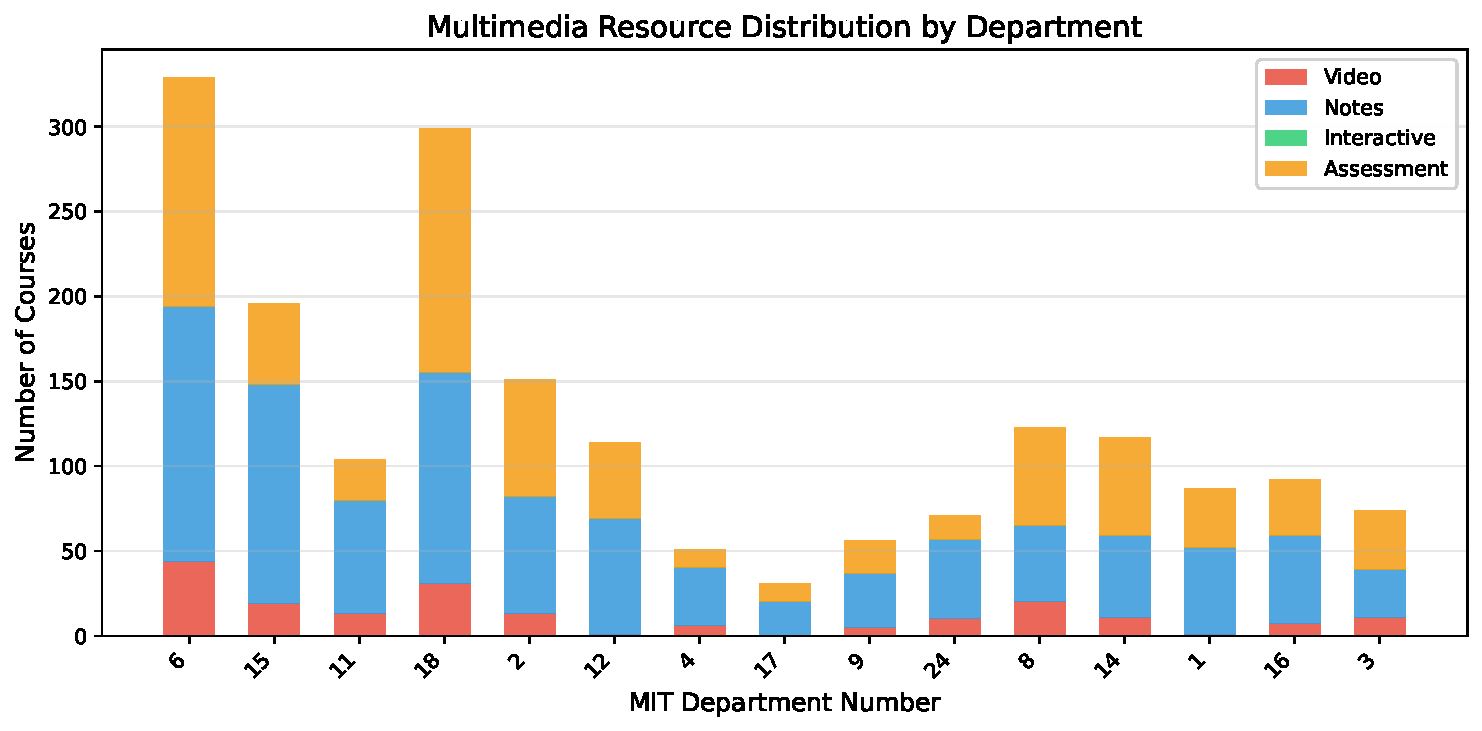
\includegraphics[width=\columnwidth]{figures/fig1_resource_distribution.pdf}
  \vspace{-2mm}
  \caption{Multimedia resource distribution by MIT department. EECS (dept.\ 6) and Mathematics (dept.\ 18) show the highest multimedia richness; departments vary in their reliance on video vs.\ notes.}
  \label{fig:resource-dist}
  \vspace{-2mm}
\end{figure}

\begin{figure}[t]
  \centering
  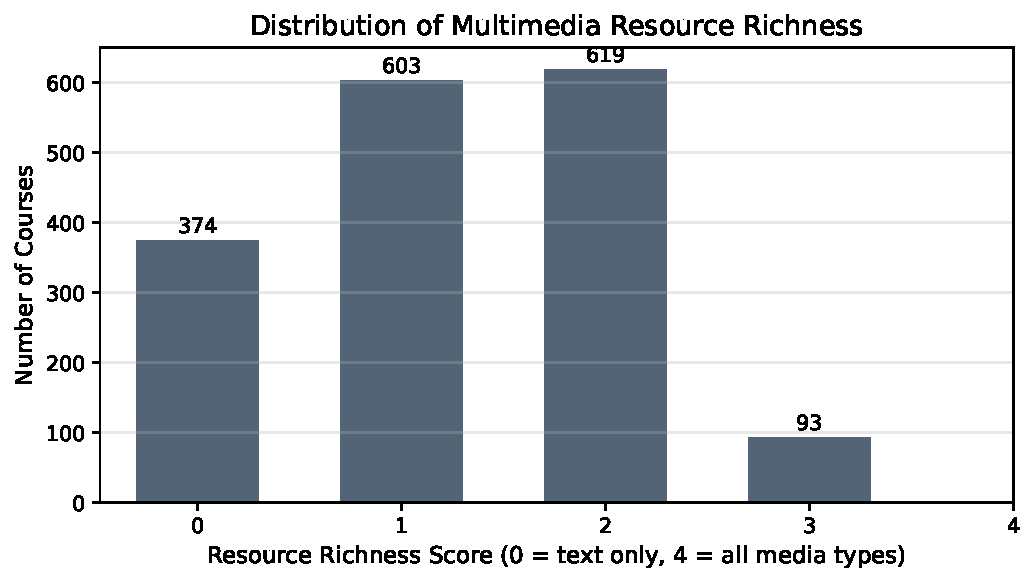
\includegraphics[width=\columnwidth]{figures/fig2_richness_histogram.pdf}
  \vspace{-2mm}
  \caption{Distribution of resource richness scores across {\NumOCWFetched} MIT OCW courses.}
  \label{fig:richness-hist}
  \vspace{-2mm}
\end{figure}

Resource type co-occurrence reveals pedagogical patterns: courses with lecture videos nearly always also provide lecture notes, but the reverse does not hold (Figure~\ref{fig:cooccurrence}).
This asymmetry creates a structured prediction challenge: textual features may predict notes availability but struggle with rarer types.

\begin{figure}[t]
  \centering
  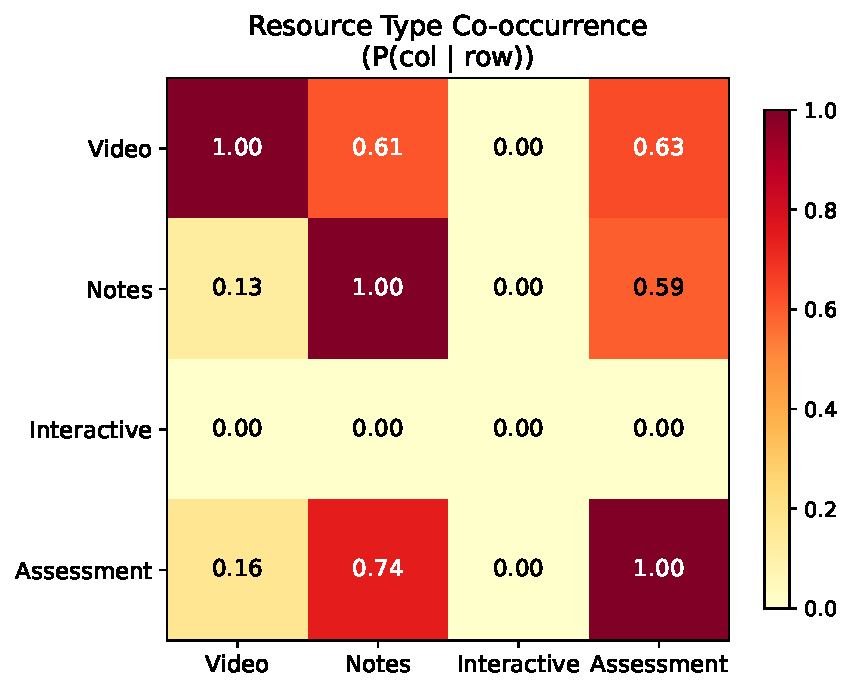
\includegraphics[width=0.85\columnwidth]{figures/fig4_cooccurrence.pdf}
  \vspace{-2mm}
  \caption{Resource type co-occurrence matrix (conditional probability). Courses with video almost always have notes (P(notes$|$video) $\approx$ 1.0), but many notes-only courses lack video.}
  \label{fig:cooccurrence}
  \vspace{-2mm}
\end{figure}

\subsection{Cross-Modal Baselines}

We evaluate two baseline approaches on the cross-modal tasks using {\JoinedCourses} courses with both text descriptions and multimodal annotations (80/20 train/test split, seed=42).

\paragraph{Department prior.}
Per-department mean prediction for richness; majority-class per department for classification.

\paragraph{TF-IDF + linear models.}
TF-IDF features (5,000 terms) from course descriptions, with ridge regression ($\lambda{=}1.0$) for richness prediction and per-label logistic regression for classification.

%%% Results table
\begin{table}[t]
\centering
\small
\caption{Cross-modal baseline results. TF-IDF features from course text predict multimedia richness with Spearman $\rho{=}{\RichnessRho}$, substantially above the department-prior baseline.}
\label{tab:baselines}
\begin{tabular}{@{}llcc@{}}
\toprule
\textbf{Task} & \textbf{Method} & \textbf{MAE $\downarrow$} & \textbf{Spearman $\rho$ $\uparrow$} \\
\midrule
\multirow{2}{*}{Richness pred.} & Department prior & {\DeptMAE} & {\DeptRho} \\
 & TF-IDF + Ridge & \textbf{\RichnessMAE} & \textbf{\RichnessRho} \\
\bottomrule
\end{tabular}
\end{table}

\paragraph{Key finding: text predicts multimedia structure.}
TF-IDF features achieve $\rho{=}{\RichnessRho}$ on richness prediction (Table~\ref{tab:baselines}), a 42\% improvement over the department-prior baseline ($\rho{=}{\DeptRho}$).
This demonstrates that course text descriptions carry meaningful signal about multimedia resource availability beyond what departmental affiliation alone provides.

Per-label classification is challenging due to class imbalance (video: 15.3\% positive, notes: 64.0\%, assessment: 46.6\%): simple logistic regression defaults to majority prediction for minority classes.
This establishes a clear baseline and motivates more sophisticated approaches (class-weighted losses, BERT-based classifiers, curriculum-aware models).

\subsection{Discussion}

The combination of high richness prediction accuracy and low per-label classification F$_1$ reveals an interesting structure: the \emph{total amount} of multimedia resources is predictable from text, but the \emph{specific types} are harder to determine.
This suggests that course descriptions encode information about instructional investment (richness) more reliably than specific pedagogical choices (video vs.\ notes vs.\ interactive).

\paragraph{Limitations of baselines.}
Our baselines use bag-of-words features; pretrained language models (BERT, GPT) would likely improve classification.
We do not evaluate cross-institutional transfer due to the single-institution annotation constraint; this remains an open task for the community.


\section{Limitations, Ethics, and Availability}
\label{sec:limitations}

\paragraph{Limitations.}
\ADSMM's multimodal annotations cover MIT OCW only; extending to other institutions requires equivalent open metadata, which most universities do not provide.
Resource type annotations capture \emph{availability}, not content quality or usage---a course marked as having video may have 2 or 40 lectures.
The cross-institutional transfer task uses MIT as the only training source, limiting generalization claims.
Course descriptions vary in quality and length across sources.

\paragraph{Geographic and linguistic bias.}
The dataset has geographic bias: 68\% of courses are from US universities, and all text is English.
O*NET reflects US labor market structure.
International representation (KTH, Edinburgh) is limited to two institutions.

\paragraph{Ethical considerations.}
All data is from public sources (university catalogs, OCW, O*NET).
No personally identifiable information is included.
MIT OCW content is licensed under CC BY-NC-SA 4.0; O*NET is public domain.
University catalog data is publicly accessible.

\paragraph{Dataset availability.}
The complete dataset, collection scripts, and evaluation code are available at \url{https://doi.org/10.5281/zenodo.18522759} (dataset) and will be released on GitHub (code).
The supplementary website provides interactive exploration of the multimodal annotations.

\paragraph{Maintenance plan.}
We commit to annual updates incorporating new OCW releases and expanded multimodal annotations.
The collection pipeline is fully automated and reproducible.


\section{Conclusion}

We presented \ADSMM, a multimodal cross-national educational resource dataset that augments {\NumCourses} course descriptions from {\NumUniversities} universities with structured multimedia resource annotations from MIT OpenCourseWare.
By capturing which courses include video, notes, interactive materials, and assessments, \ADSMM enables cross-modal analysis at a scale not previously possible in educational data mining.
Our three evaluation tasks---multimedia richness prediction, resource type classification, and cross-institutional transfer---provide standardized benchmarks for the multimedia education research community.

Initial baselines show that course text descriptions carry meaningful signal about multimedia structure, but significant room for improvement remains, particularly for cross-institutional transfer.
We release all data, code, and baselines to support reproducible research at the intersection of multimedia and education.


%% ===========================================================================
%% BIBLIOGRAPHY
%% ===========================================================================

\bibliographystyle{ACM-Reference-Format}
\bibliography{references}

\end{document}
